\chapter{Desempe\~no del programa original}
\label{ch:prev_work}

A continuaci\'on se exponen los resultados de diferentes pruebas realizadas sobre el programa original con la finalidad de medir su desempe\~no computacional en t\'erminos de tiempo de ejecuci\'on y uso de memoria.
\bigskip

Estas pruebas se llevaron a cabo en un computador personal de 8 GB (DDR4) de RAM. La raz\'on de esta  medida (que no se hayan ejecutado en Leftraru) tuvo que ver con que el c\'odigo original contiene demasiadas l\'ineas con el comando \texttt{glob}\footnote{\url{https://docs.python.org/3.5/library/glob.html}} de Python el cual lista reiteradamente el contenido de los directorios de los archivos lo que finalmente termina saturando el nodo destinado para el lanzamiento del programa (en Leftraru el programa no se ejecuta de la misma forma que lo har\'ia localmente, ya que recorre la lista de 93 supernovas de HiTS, repitiendo para cada una de ellas el mismo proceso). Por esto \'ultimo, los administradores del sistema del NLHPC sugirieron modificaciones al programa original, sin embargo, en pos de continuar con el esp\'iritu de esta tesis, se opt\'o por efectuar los experimentos de manera local (usando un computador personal) evitando as\'i introducir m\'as modificaciones (se adapt\'o el programa para Python 3.5, ya que originalmente estaba para 2.7 agregando cambios menores como la forma de imprimir mensajes en consola (\texttt{print})).
\bigskip


Cabe destacar que el problema anteriormente descrito comenz\'o a presentarse una vez que el autor original del mismo pudo corregir la revisi\'on de los nuevos candidatos en el mes de Junio del presente a\~no, debido a que la primera versi\'on del programa s\'olo estaba verificando la presencia de una supernova conocida y no estaba revisando los potenciales nuevos candidatos. Esto se agreg\'o como una continuaci\'on del programa repitiendo pasos como el c\'alculo de flujos, calculo de matrices de estados y sus respectivas predicciones usando alg\'un tipo de filtro de Kalman, etc. El diagrama de la figura \ref{fig:des_sif} entrega una perspectiva general de la secuencia de pasos que realiza el programa.
\bigskip

\begin{figure}[h!]
\centering
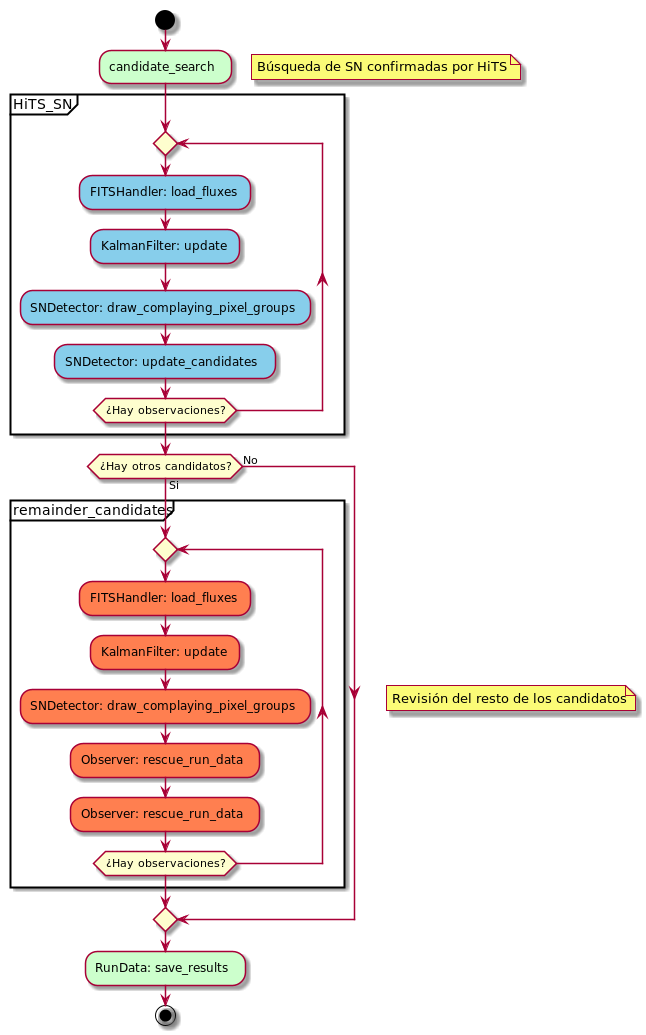
\includegraphics[scale=.5]{images/results/sif_act}
\caption{Diagrama de actividad del programa original. Se aprec\'ian dos ciclos principales: el primero est\'a destinado a la b\'usqueda de una supernova de HiTS, y el segundo a la revisi\'on de la lista de posibles candidatos encontrados durante la verificaci\'on de la supernova de HiTS. Notar que hay pasos que se repiten en la realizaci\'on de ambos an\'alisis.}
\label{fig:des_sif}
\end{figure}

\section{Tiempo de ejecuci\'on}

El estudio del tiempo de ejecuci\'on del programa se realiz\'o usando la funci\'on \texttt{getrusage} de la librer\'ia \texttt{resource} de Python, midiendo el tiempo de usuario en segundos. Las mediciones se realizaron sobre tres conjuntos de datos (las cuales contienen alguna supernova detectada por HiTS) seleccionados al azar: SN14, SN18 y  SN80. En cada uno de ellos comprende secuencias de 26 observaciones. 

\begin{table}[h]
\centering
\begin{tabular}{|l|l|l|l|l|}
\hline
\textbf{ID} & \textbf{C\'alc. Flujos [s]} & \textbf{Aplic. KF [s]} &  \textbf{Agrup. Pixeles [s]}  & \textbf{Actual. Candidatos [s]}\\ \hline \hline
SN14        & 320.98            & 29.39        &  39.98 & 0.01 \\ \hline
SN18            & 290.48             & 23.89         &  36.64  & 0.01\\ \hline
SN80            & 297.79             & 25.40         &   36.88 & 0.01 \\ \hline \hline
Media & 303.08 &  26.23 & 37.83 & 0.01\\\hline 
$\bar{t}/Obs$ & 11.66 &  1.01 & 12.61 & 0.00\\\hline 
\end{tabular}
\label{tab:t1}
\caption{Resultados de tiempos de ejecuci\'on correspondientes a calculo de flujos, estimaci\'on de los filtros, agrupaci\'on de pixeles y filtrado de los mismos durante el peri\'odo de reconocimiento de la supernova correspondiente. Para esta prueba se utiliz\'o el filtro de Kalman B\'asico.}
\end{table}

\begin{table}[h]
\centering
\begin{tabular}{|l|l|l|l|l|}
\hline
\textbf{ID} & \textbf{C\'alc. Flujos [s]} & \textbf{Aplic. KF [s]} &  \textbf{Agrup. Pixeles [s]}  & \textbf{Guardar resultados [s]}\\ \hline \hline
SN14        & 333.59            & 36.13        &  42.22 & 0.09 \\ \hline
SN18            & 289.45             & 24.15         &  36.87  & 0.05\\ \hline
SN80            & 297.90             & 26.39         &   37.59 & 0.06 \\ \hline\hline 
Media & 306.98 &  28.89 & 38.89  & 0.07\\\hline 
$\bar{t}/Obs$ & 11.81 &  1.11 & 1.50 & 0.00\\\hline 
\end{tabular}
\label{tab:t2}
\caption{Resultados de tiempos de ejecuci\'on correspondientes a calculo de flujos, estimaci\'on de los filtros, agrupaci\'on de pixeles y filtrado de los mismos durante el peri\'odo de estudio de los nuevos candidatos encontrados en el paso anterior. Para esta prueba se utiliz\'o el filtro de Kalman B\'asico.}
\end{table}


\begin{table}[h]
\centering
\begin{tabular}{|l|l|l|l|l|}
\hline
\textbf{ID} & \textbf{C\'alc. Flujos [s]} & \textbf{Aplic. KF [s]} &  \textbf{Agrup. Pixeles [s]}  & \textbf{Actual. Candidatos [s]}\\ \hline \hline
SN14        & 327.92            & 731.98        &  38.42 & 0.01 \\ \hline
SN18            & 290.05             & 554.62         &  35.00  & 0.00\\ \hline
SN80            & 309.98             & 628.83         &   37.80 & 0.01 \\ \hline \hline 
Media & 309.32 & 638.48 &  37.07 & 0.01\\\hline
 $\bar{t}/Obs. $& 11.90 & 24.56 & 1.43 & 0.00\\\hline 
\end{tabular}
\label{tab:t3}
\caption{Resultados de tiempos de ejecuci\'on correspondientes a calculo de flujos, estimaci\'on de los filtros, agrupaci\'on de pixeles y filtrado de los mismos durante el peri\'odo de reconocimiento de la supernova correspondiente. Para esta prueba se utiliz\'o el filtro de Kalman de M\'axima Correntrop\'ia.}
\end{table}

\begin{table}[h]
\centering
\begin{tabular}{|l|l|l|l|l|}
\hline
\textbf{ID} & \textbf{C\'alc. Flujos [s]} & \textbf{Aplic. KF [s]} &  \textbf{Agrup. Pixeles [s]}  & \textbf{Guardar resultados [s]}\\ \hline \hline
SN14        & 302.28            & 631.17        &  36.98 & 0.04 \\ \hline
SN18            & 311.63             & 660.51         &  35.68  & 0.06\\ \hline
SN80            & 306.22             & 610.60         &   36.37 & 0.04 \\ \hline \hline
Media & 306.71 & 634.09 &  36.34 & 0.05\\\hline
 $\bar{t}/Obs. $& 11.80 & 24.39 & 1.40 & 0.00\\\hline  
\end{tabular}
\label{tab:t4}
\caption{Resultados de tiempos de ejecuci\'on correspondientes a calculo de flujos, estimaci\'on de los filtros, agrupaci\'on de pixeles y filtrado de los mismos durante el peri\'odo de estudio de los nuevos candidatos encontrados en el paso anterior. Para esta prueba se utiliz\'o el filtro de Kalman de M\'axima Correntrop\'ia.}
\end{table}

\begin{table}[h]
\centering
\begin{tabular}{|l|l|l|l|}
\hline
\textbf{ID} & \textbf{B\'usqueda SN} & \textbf{Revisi\'on candidatos} & \textbf{Tiempo total} \\ \hline
\hline
SN14 & 390.36 & 412.03 & 802.39 \\\hline
SN18 & 351.02 & 350.52 & 701.54\\\hline
SN80 & 360.08 & 361.94 & 722.02 \\\hline\hline
Media & 367.15 & 374.83 & 741.98  \\\hline
 $\bar{t}/Obs. $& 14.12 & 14.42 & 28.54\\\hline 
\end{tabular}
\label{tab:t5}
\caption{Tiempo de ejecuci\'on de los procesos de b\'usqueda de supernova de HiTS, revisi\'on de los candidatos encontrados y tiempo total comprendido por ambos procesos usando filtro de Kalman B\'asico.}
\end{table}


\begin{table}[h]
\centering
\begin{tabular}{|l|l|l|l|}
\hline
\textbf{ID} & \textbf{B\'usqueda SN} & \textbf{Revisi\'on candidatos} & \textbf{Tiempo total} \\ \hline
\hline
SN14 & 1098.33 & 970.47 & 2068.80\\\hline
SN18 & 879.67 & 1007.88 & 1887.55\\\hline
SN80 & 976.62& 953.23& 1929.85\\\hline \hline
Media & 367.15 & 374.83 & 741.98  \\\hline
 $\bar{t}/Obs. $& 14.12 & 14.42 & 28.54\\\hline 
\end{tabular}
\label{tab:t6}
\caption{Tiempo de ejecuci\'on de los procesos de b\'usqueda de supernova de HiTS, revisi\'on de los candidatos encontrados y tiempo total comprendido por ambos procesos usando filtro de Kalman de M\'axima correntrop\'ia.}
\end{table}

\section{Uso de memoria}

La memoria ocupada por el programa se midi\'o en t\'erminos de MiB (Mebibyte) usando la librer\'ia \texttt{memory\_profiler}. Posteriormente las mediciones en la unidad previamente mencionada fueron pasadas a MB\footnote{$1MiB\simeq 1.049$ }

\begin{figure}[h!]
\centering
\subfloat[Memoria ocupada en SN14]{\label{fig:kbf_14}{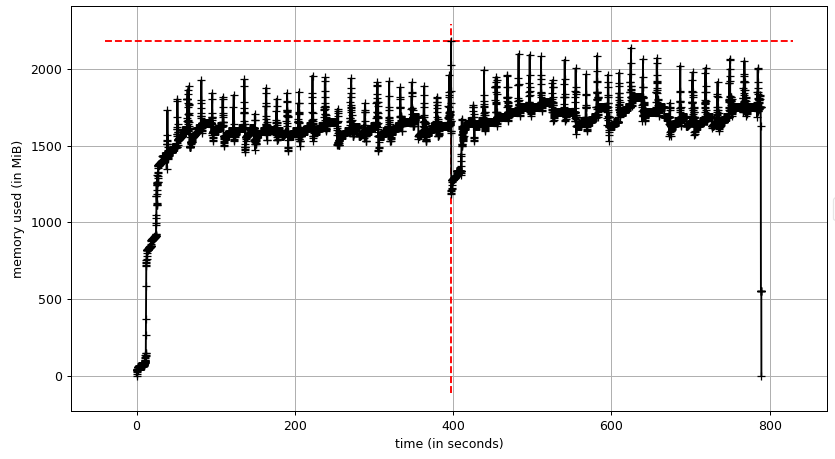
\includegraphics[width=0.5\textwidth]{images/results/sn14_00}}}\hfill
\subfloat[Memoria ocupada en SN18]{\label{fig:kbf_18}{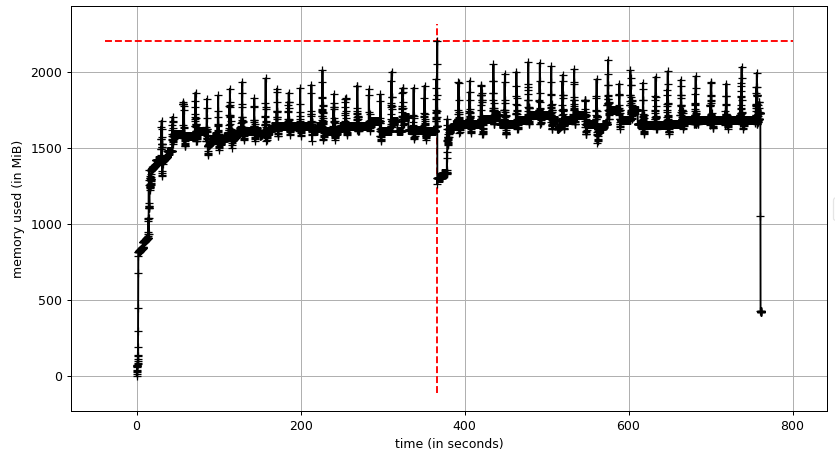
\includegraphics[width=0.5\textwidth]{images/results/sn18_00}}}\vfill
\subfloat[Memoria ocupada en SN80]{\label{fig:kbf_80}{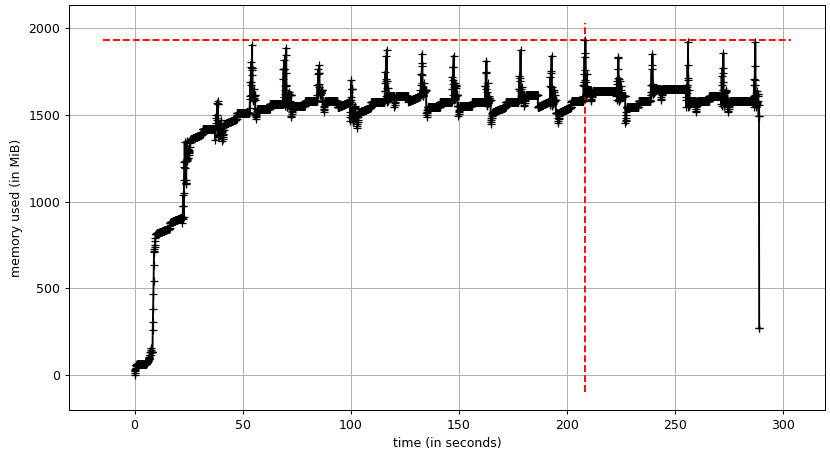
\includegraphics[width=0.5\textwidth]{images/results/sn80_00}}}
\caption{Comportamiento de la memoria (en mebibytes) durante la ejecuci\'on para los tres conjuntos de datos. En los tres lanzamientos se us\'o el filtro de Kalman B\'asico.}
\label{fig:mem_kbf}
\end{figure}

\begin{table}
\centering
\begin{tabular}{|l|l|}
\hline
\textbf{ID} & Memoria [MB]\\\hline\hline
SN14 & 2290.10\\\hline
SN18 & 2314.17\\\hline
SN80 & 2191.82\\\hline
\end{tabular}
\caption{Memoria principal (en unidades de MB) usada durante la ejecuci\'on del programa original usando la versi\'on b\'asica del filtro de Kalman.}
\label{tab:mem1}
\end{table}

\begin{figure}[h!]
\centering
\subfloat[Memoria ocupada en SN14]{\label{fig:mc_14}{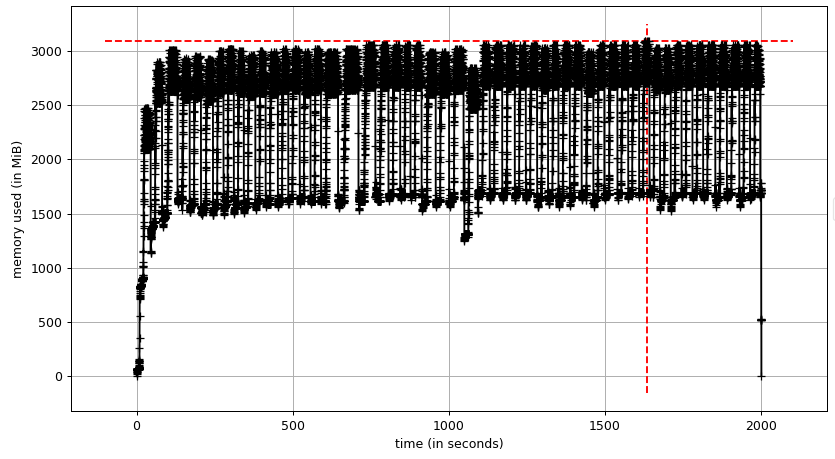
\includegraphics[width=0.5\textwidth]{images/results/sn14_01}}}\hfill
\subfloat[Memoria ocupada en SN18]{\label{fig:mc_18}{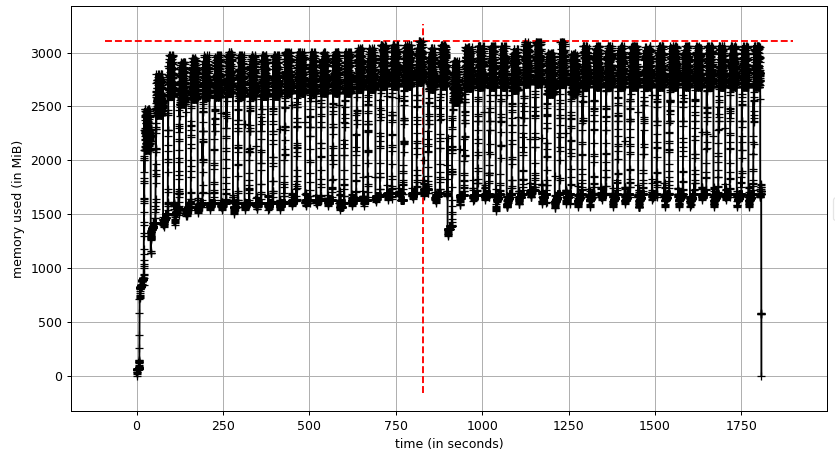
\includegraphics[width=0.5\textwidth]{images/results/sn18_01}}}\vfill
\subfloat[Memoria ocupada en SN80]{\label{fig:mc_80}{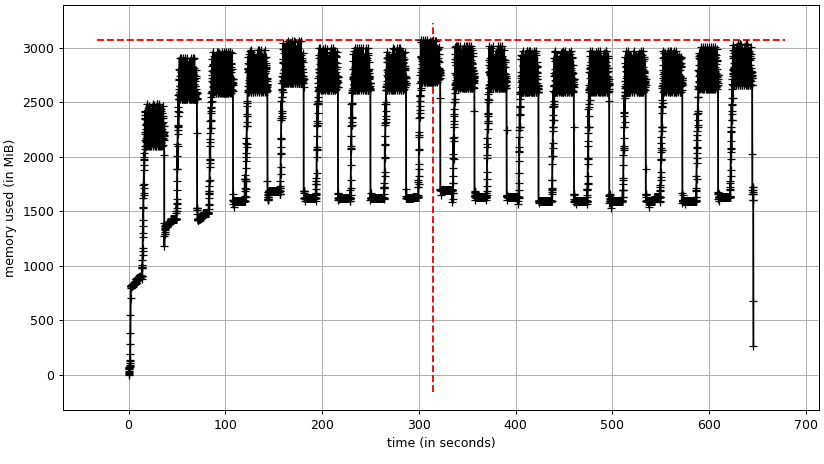
\includegraphics[width=0.5\textwidth]{images/results/sn80_01}}}
\caption{Comportamiento de la memoria (en mebibytes) durante la ejecuci\'on para los tres conjuntos de datos. En los tres lanzamientos se us\'o el filtro de Kalman de correntrop\'ia m\'axima.}
\label{fig:mem_mcc}
\end{figure}

\begin{table}
\centering
\begin{tabular}{|l|l|}
\hline
\textbf{ID} & Memoria [MB]\\\hline\hline
SN14 & 3320.12\\\hline
SN18 & 3248.78\\\hline
SN80 & 3320.12\\\hline
\end{tabular}
\caption{Memoria principal (en unidades de MB) usada durante la ejecuci\'on del programa original usando filtro de Kalman de m\'axima correntrop\'ia.}
\label{tab:mem2}
\end{table}

